\chapter{Proposta de Algoritmo}
\label{algorithm-proposition}

Neste capítulo será apresentado o algoritmo que este trabalho visa propor e detalhes de seu funcionamento e vantagens.

\section{Motivação}
\label{motivation}

A evolução no campo da criptografia é constante e há sempre novas propostas de algoritmos que focam em solucionar um obstáculo imposto por possíveis atacantes e seus métodos para se obter informações sigilosas.

O algoritmo proposto neste trabalho visa diminuir as possibilidades de análises de frequência de um texto cifrado. É uma nova modalidade na produção de texto cifrado utilizando cifra de fluxo. 


\section{Funcionamento}
\label{functioning}

O algoritmo terá como entrada uma sequência de números pseudo-aleatórios e terá como objetivo produzir um texto cifrado onde as frequências de ocorrência dos caracteres é totalmente balanceada.

A cada \textit{byte} de texto em claro será feito um ou-exclusivo com o número na posição correspondente da sequência e com isso vai se preenchendo uma tabela de equalização de \textit{bytes} que tem posições de 0 a 255.

\begin{figure}[h]
	\centering
	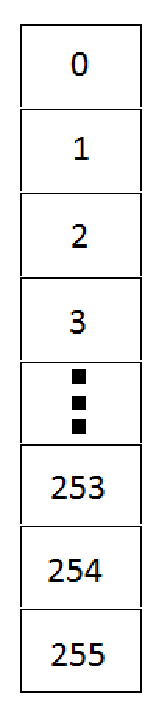
\includegraphics[scale=0.7]{figuras/tabela.eps}
	\caption{Tabela de \textit{byte} para uso do algoritmo}
\end{figure}

Como o resultado deverá ser totalmente balanceado, há a possibilidade de se produzir um resultado em uma posição na tabela já ocupada, para contornarmos esse problema, propomos a seguinte solução: a introdução da variável \textbf{j} e um \textit{byte} da tabela de equalização que servirá para indicar que houve um conflito na cifra e se chamará de \textbf{sinal}.

\begin{figure}[h]
	\centering
	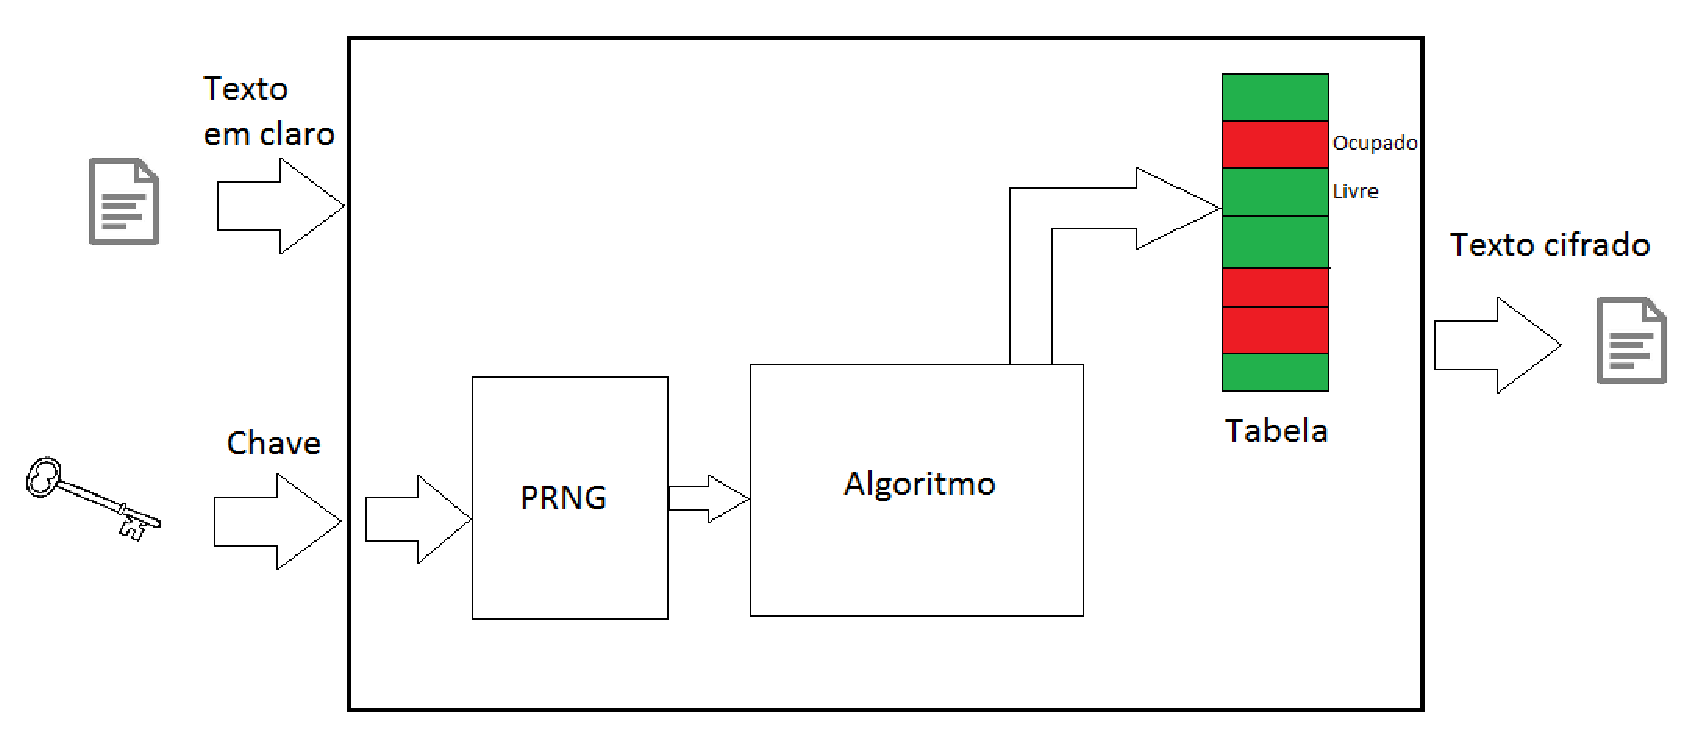
\includegraphics[scale=0.6]{figuras/funcionamento.eps}
	\caption{Esquema do algoritmo de cifração}
\end{figure}

A variável \textbf{j} visa quantificar os números pseudo-aleatórios que deverão ser descartados na produção do texto cifrado e com isso o receptor da mensagem terá a possibilidade de recuperar a mensagem original com sucesso. O processo de cifração que pode ser visto no pseudo-código na figura \ref{pseudo-codigo} segue os seguintes caminhos:

\begin{figure}[h]
	\centering
	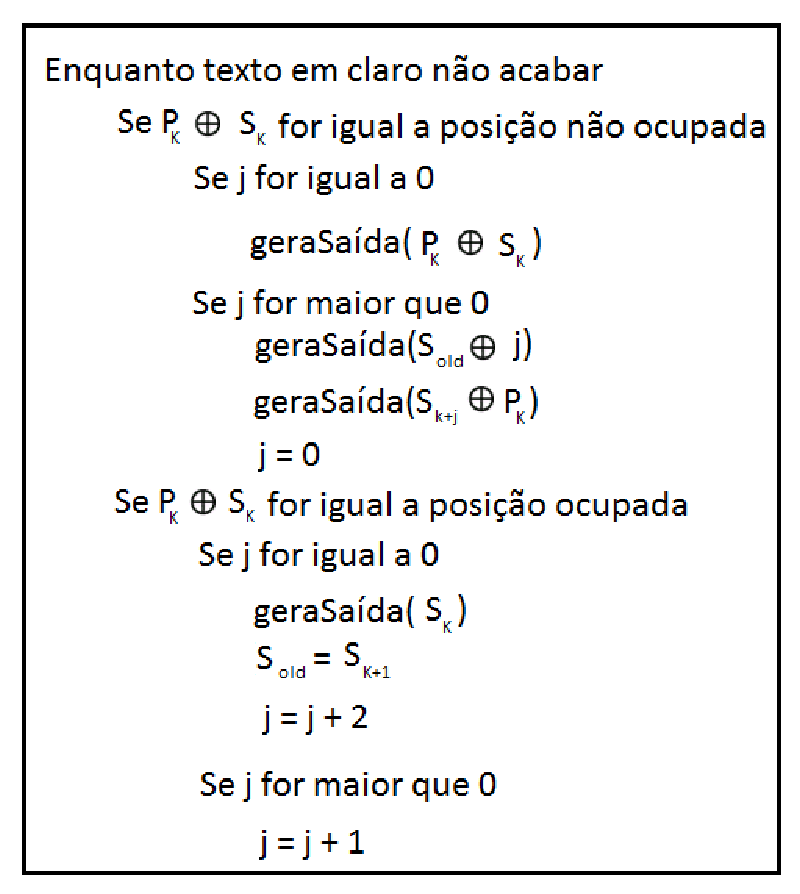
\includegraphics[scale=1]{figuras/pseudocondigo.eps}
	\caption{Pseudo código do algoritmo de cifração}
	\label{pseudo-codigo}
\end{figure}

O caminho ideal é o que o resultado da operação ou-exclusivo entre o \textit{byte} do texto em claro e o número aleatório correpondente sempre seja igual a uma posição livre na tabela de balanceamento.

Caso se detecte um conflito de resultados na tabela de balanceamento, é enviado o sinal para o receptor da mensagem, pois com isso o receptor saberá que o próximo valor recebido será a quantidade de números pseudo-aleatórios que deverão ser descartados da sequência.Esse sinal irá ser cifrado com o valor do número aleatório que gerou o conflito Então o algoritmo vai executar o comando de descartar os números pseudo-aleatórios, até que se encontre um resultado em uma posição que esteja livre na tabela de balanceamento. Ao encontrar essa posição livre, o algoritmo deverá enviar o resultado do ou-exclusivo entre j(quantidade de números descartados) e S$_{old}$ e o valor de j é novamente estabelecido como 0.

Quando a tabela for totalmente concluída, o processo se inicia de novo e suas posições ficam livres com exceção do novo sinal e o algoritmo continua com o processo de preenche-la novamente. Esse processo só finaliza quando os bytes do texto em claro forem todos cifrados. O processo de estabelecer o valor do sinal será feito da seguinte forma:

\begin{enumerate}
	\item Para a primeira rodada\footnote{Processo de completar a tabela de equalização.}, o sinal será o primeiro valor produzido pelo gerador de números aleatórios.
	\item A partir da segunda rodada, o sinal será o último \textit{byte} cifrado da rodada anterior. 
\end{enumerate}

\begin{figure}[h]
	\centering
	\includegraphics[scale=0.6]{figuras/metodo_de_decifra.eps}
	\caption{Esquema do algoritmo de decifração}
\end{figure}

Podemos observar o processo de decifrar na figura \ref{pseudo-codigo-decifrar}. É um processo diferente do processo de cifrar, pois não inclui a tabela de balanceamento e assim o processo de balanceamento não se faz necessário. Portanto, para decifrar é necessário ter a capacidade de produzir a mesma sequência de números aleatórios e, portanto, ter a mesma chave que foi utilizada no processo de cifrar. 


\begin{figure}[h]
	\centering
	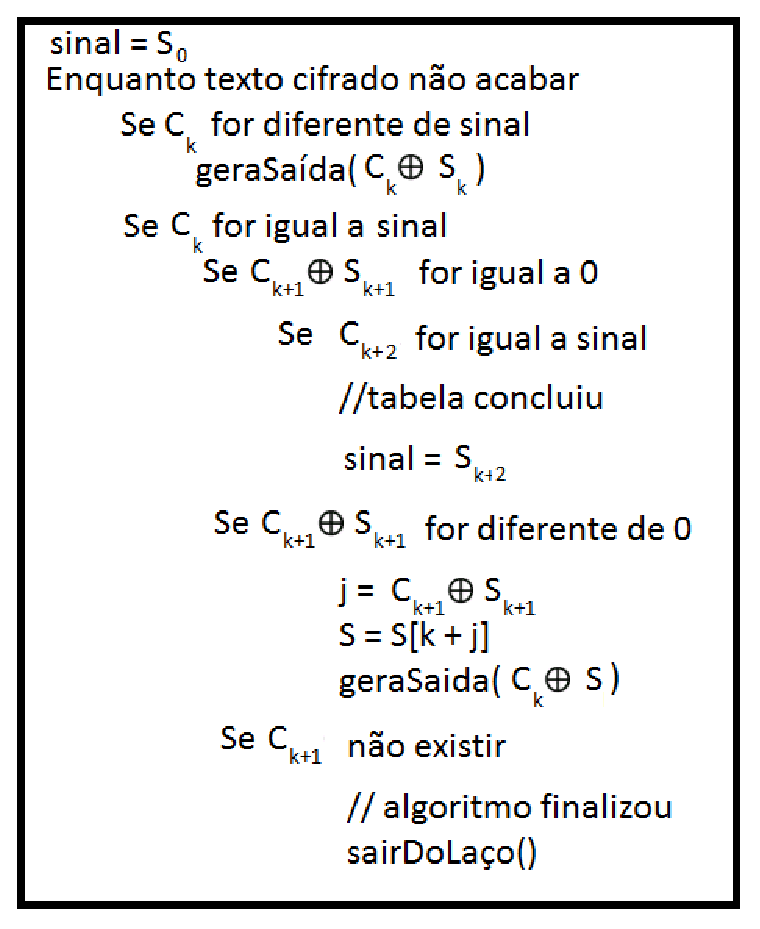
\includegraphics[scale=1]{figuras/funcionamento_Decifra.eps}
	\caption{Pseudo código do algoritmo de decifração}
	\label{pseudo-codigo-decifrar}
\end{figure}

O primeiro passo da decifração é realizar a função ou-exclusivo entre o \textit{byte} do texto cifrado e o número aleatório correspondente. O caminho ideal é que o resultado dessa operação seja diferente de zero, pois assim, esse resultado é o \textit{byte} do texto em claro.

Se o resultado da operação ou-exclusivo entre \textit{byte} do texto cifrado e o número aleatório for igual a \textit{byte} que foi denominado para aquela rodada ser o sinal, isso quer dizer que o próximo \textit{byte} do texto cifrado será o resultado da variável \textbf{j}, que indica quantos números aleatórios devem ser descartados para o processo de decifração. Ao se descartar esses números, o processo volta para o percurso normal de execução. 

A maior vantagem desse algoritmo é que por ser muito genérico, isso resulta que não importa qual gerador de números pseudo-aleatório será utilizado. Outra vantagem é que a utilização desse algoritmo pode ser combinada com outro algoritmo de cifração de fluxo, aumentando a segurança do texto cifrado.